\chapter{Metodologia}
\label{chap:metodologia}

Para o desenvolvimento desse projeto, foi utilizado o ROS \textit{Kinetic}, considerado uma das versões mais estáveis ROS. Ele é compatível apenas com o Ubuntu 16.04, tornando necessário a instalação do mesmo em \textit{dual boot}, mantendo o sistema operacional \textit{Windows} como segunda opção de \textit{boot}.

A comunicação com o Jaguar é feita através de uma rede \textit{wireless}. Nessa rede terá um \textit{node} do ROS que controla a aceleração e o ângulo de rotação da plataforma. É possível acessá-lo conectando um dispositivo na mesma rede do Jaguar e um \textit{node master}, que é um \textit{node} que tem o endereço de todos os outros dispositivos conectados a rede. Com um computador é possível criar o \textit{master} e mais quantos outros \textit{nodes} for preciso no mesmo dispositivo.

Com o computador conectado a rede \textit{wireless} do Jaguar e os \textit{nodes} do ROS funcionando, é possível configurar um controle remoto para a plataforma. Esse controle trás uma praticidade e uma precisão para gerar dados que o teclado do computador não possui. O PC cria um novo \textit{node} na rede que enviará comandos ao \textit{node} de aceleração e rotação da plataforma. 

Para fazer a navegação autônoma do Jaguar por apenas uma câmera é preciso primeiro ter um modelo treinado com dados constituídos de imagens e seus respectivos valores de angulação e aceleração capturas pela plataforma. Esses dados precisam ser de algum percurso onde o Jaguar foi controlado por uma pessoa, já que o algoritmo de CNN precisa ter uma base de dados para criar o modelo.

Os dados de treinamento são obtidos enquanto o Jaguar é controlado por controle remoto executando o arquivo \textit{Savefile.py}. Seu funcionamento é explicado na sessão \ref{sec:Savefile.py} e é preciso que o Jaguar seja controlado com muito cuidado e atenção para obter dados de qualidade.

O modelo é feito pelo \textit{Model.py}. Ele cria vário modelos de acordo com o valor de \textit{epoch}, que determina essa quantidade, mas o modelo seguinte só será criado se o seu \textit{val\_loss} for menor que o modelo anterior. Esse \textit{val\_loss} é exibido na tela de execução do arquivo e mostra o erro do modelo feito no teste simulado. Quando o \textit{model.py} vai criar o modelo ele separa 80\% das imagens para o treinamento e 20\% para o teste do modelo criado. O \textit{val\_loss} mostra o erro do teste, por isso esse valor precisa ser o menor possível.

O algoritmo de Rede Neural Convolucional é mesmo utilizado no projeto \textit{Car Behavioral Cloning} \cite{naokish}. E o python, linguagem computacional dos arquivos desse projeto, é utilizada para o desenvolvimento da CNN e também é incluída nativamente no ROS, facilitando toda a integração do projeto. Por isso o uso dela.

Com o modelo gerado e a conexão \textit{wireless} com o Jaguar estabelecida é possível colocar a plataforma para testar os modelos de navegação autônoma. O arquivo \textit{drive.py} realiza o controle autônomo da plataforma e ele foi programado para ser executado no \textit{terminal} do Linux ao lado do modelo escolhido para o treinamento. Através da rede \textit{wireless} o \textit{drive.py} se conecta a câmera IP do Jaguar e captura as imagens, faz todo o processamento com cada uma delas e envia para o \textit{node} da rede o respectivo valor de aceleração e angulação de cada uma. 

Todos esses programas são essenciais para o funcionamento do projeto e serão explicados com mais detalhes na sessão \ref{sec:programas essenciais}.

%%%%%%%%%%%%%%%%%%%%%%%%%%%%%%%%%%%%%%%%%%%%%%%%%%%%%%%%%%%%%%%%%%%%%%%%%

\section{programas essenciais}
\label{sec:programas essenciais}
Há quatro programas essenciais para o funcionamento do projeto: \textit{savefile.py, Model.py, Utils.py} e \textit{Drive.py}. Eles são todos programados em python e cada um desses arquivos desempenha uma função única e fundamental para o perfeito funcionamento do sistema autônomo no jaguar.

\subsection{\textit{Savefile.py}}
\label{sec:Savefile.py}

É o primeiro arquivo a ser executado. Ele foi criado pelo autor do projeto com o intuito de salvar as imagens capturadas pelo Jaguar e criar o arquivo \textit{driver\_log.csv} que contém a localização de cada uma das imagens juntamente com o ângulo de rotação e valor de aceleração do exato momento de captura. 

Esse arquivo deve ser executado enquanto o piloto controla o Jaguar para adquirir os dados de análise (no caso, o \textit{driver\_log.csv} e as imagens) e, de preferência, que seja obtido um grande número de dados para a criação de um bom modelo. 

O \textit{Savefile.py} possui bibliotecas como ''cvs'' e ''os'' para tratamento dos dados e ''rospy'' e ''twist'' para criar um \textit{node} do ROS na rede do Jaguar e receber os dados de angulação e rotação enviados pelo piloto. Para receber esse dados, há um método dentro do arquivo chamado de \textit{listener()} que recebe todos os valores enviados para o \textit{node} de movimentação do Jaguar. Assim que o valor muda, é chamado o método \textit{salvarArquivos()} para abrir o arquivo .csv e salvar os dados e as imagens capturadas no exato instante de movimentação do Jaguar.

\subsection{\textit{Model.py}}
\label{sec:model.py}

É o arquivo de criação de modelo. 
Ele foi desenvolvido pelo a Udacity e adaptado para esse projeto com intuito de criar um modelo de predição para o Jaguar a partir do arquivo \textit{driver\_log.csv}. Ele abre esse arquivo e divide seus dados entre dados de treinamento (80\% dos dados) e dados de teste (20\% dos dados). Os dados de treino são usados para criar o modelo da rede neural e os dados de teste são para testar esse modelo. O método de criação do arquivo \textit{model.py} é mostrado na Figura \ref{model3}.

	\begin{figure}[H]
		\centering
		\Caption{\label{model3}Linhas de código do 37 à 54 arquivo model.py}
		\UNIFORfig{}{
			\fbox{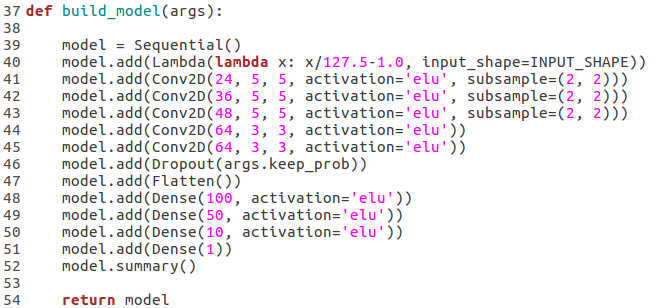
\includegraphics[width=16cm]{fig/12.png}}
		}{
			\Fonte{Elaborado pelo autor}
		}	
\end{figure}

A rede neural do projeto é mostrada Figura \ref{model3} e inicia com um espaço em branco na memória para o Keras trabalhar, na linha 39. 
Na linha 40, é adicionado uma camada de normalização de imagem. O número 127.5-1.0 foi escolhido pela comunidade de desenvolvedores depois de treinar com diferentes valores. Eles normalizam as imagens assim que são colocadas e evitam a saturação e fazem com que o gradiente funcione melhor. Ou seja, as imagens podem vim com sombras, de má qualidade. Essa função pode formatar e remodelar a imagem para trazer boas predições.
Nas linhas 40 à 45 são adicionadas 5 camadas convolucionais na rede neural. Ela recebe os seguintes argumentos: 

\begin{lstlisting}
conv2D(nb_filter, nb_row, nb_col, activation, subsample)
\end{lstlisting}

\begin{description}
    \item[nb\_filter:] Número de filtros de convolução a serem usados.
    \item[nb\_row:] Número de linhas no kernel da convolução.
    \item[nb\_col:] Número de colunas no kernel da convolução.
    \item[activation:] nome da função de ativação a ser usada. No caso, todas foram ELU:\textit{exponetial linear units}, usada para cuidar do problema gradiente de fuga
    \item[subsample:] tupla de comprimento 2x2. Tem a função de reduzir a imagem sem perder suas principais características.
    \item[Fonte:] \cite{kerasconv}
\end{description}
A camada de dropout, na linha 46, tem como função dar maior robustez à rede para previsões fora da amostra, buscando capturar informações populacionais ao invés de características amostrais. 
Dropout é um algoritmo relativamente novo para treinamento de redes neurais, que se fundamenta na eliminação aleatória de neurônios durante o processo de aprendizagem, para evitar a sobreadaptação aos dados (overfitting).

Na linha 47, o \textit{Flatten()} faz a preparação (achatamento) dos dados para trabalhar com series de camadas totalmente conectadas. As camadas convolucionais prepararam as imagens para serem tratadas pela rede neural. A intenção do código é achar uma relação das imagens com o \textit{steering\_angle} e o \textit{throttle}.

Da linha 48 até a linha 51 é criada a rede neural totalmente conectada. É possível observar que número de neurônios dessa rede vai reduzindo conforme a adesão de novas camadas, até chegar a um neurônio, na linha 51. 


	\begin{figure}[H]
		\centering
		\Caption{\label{model4}Linhas de código do 57 à 74 arquivo model.py}
		\UNIFORfig{}{
			\fbox{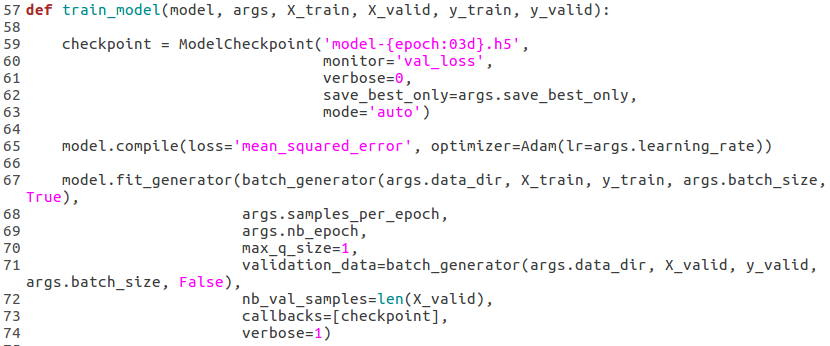
\includegraphics[width=16cm]{fig/13.png}}
		}{
			\Fonte{Elaborado pelo autor}
		}	
\end{figure}

A função \textit{train\_model()}, linha 57 da Figura\ref{model4}, tem como função treinar o modelo criado. Na linha 59, há um método que salva um modelo a cada \textit{epoch} (quantidade de vezes que o conjunto será treinado), caso ele tenha um \textit{'val\_loss'} menor que o anterior.

O Compilador do modelo, na linha 65, utiliza o método \textit{'mean\_squared\_error'}, que calcula a diferença entre o quadrado do valor esperado e o quadrado do valor obtido e tira a média de todos os valores obtidos para achar o erro. Esse método utiliza o otimizador Adam, que é um gradiente de descida.

\[\sum_{1}^{n}\frac{(valor\_real - valor\_obtido)^{2}}{n}\]

Na linha 67, o \textit{mode.fit\_generator} faz o treinamento do modelo. Ele utiliza o método \textit{batch\_generator()} do arquivo \textit{utils.py} e argumentos do \textit{main()} para fazer o treinamento e o \textit{checkpoint} da linha 59 para salvar o modelo treinado.


\subsection{\textit{Utils.py}}

 O jaguar consegue tirar fotos e gravar em alta resolução. Isso pode ser muito bom a princípio, porém imagens grandes podem aumentar ainda mais tempo de criação do modelo e predição. Então, para resolver esse problema a Udacity fornece o \textit{utils.py}: ele edita as imagens para facilitar o processamento do \textit{model.py} e \textit{drive.py}, já que o programa irá examinar \textit{pixel} por pixel de cada imagem, onde uma mudança em qualquer um dos \textit{pixels} o computador reconhece como uma nova imagem.

Esse arquivo também tem a função de gerar imagens modificadas, com o intuito de aumentar o volume de dados treinamento e teste para a rede neural.

\subsection{\textit{Drive.py}}
\label{sec:drive.py}

Esse programa foi fornecido pelo Udacity e adaptado para esse projeto. Sua função é realizar o controle autônomo do Jaguar trabalhando em conjunto com os arquivos modelo (\textit{"model-002.h5"}, por exemplo) e o \textit{utils.py}. Ele recebe as imagens do Jaguar por IP, faz o tratamento delas com o auxílio do \textit{utils.py} e retorna comandos de velocidade e angulação para o \textit{node} da rede do Jaguar. 

Esse arquivo foi modificado para receber as imagens da câmera por IP como é mostrado na linha 35 da Figura \ref{figura 8} e limitar a velocidade para a máxima do Jaguar(variável \textit{MAX\_SPEEP}: 1.0).

\begin{figure}[H]
	\centering
	\Caption{{\label{figura 8}}Linhas de código do 31 à 51 arquivo drive.py}
	\UNIFORfig{}{
		\fbox{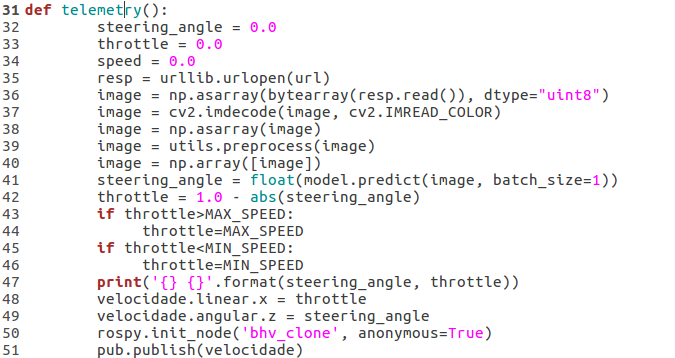
\includegraphics[width=14cm]{fig/8.png}}
	}{
		\Fonte{Elaborado pelo autor}
	}	
\end{figure}

A função \textit{telemetry()} da Figura \ref{figura 8} tem a função de receber as imagens da câmera IP do Jaguar, fazer o a predição para essa imagem e salvar os valores de aceleração e angulação nas variáveis \textit{velocidade.linear.x} e \textit{velocidade.angular.z}, respectivamente. Ao final da função, esse valores são enviados para o \textit{node} que controla a movimentação do Jaguar.